% Created by tikzDevice version 0.6.1 on 2011-06-03 22:21:24
% !TEX encoding = UTF-8 Unicode
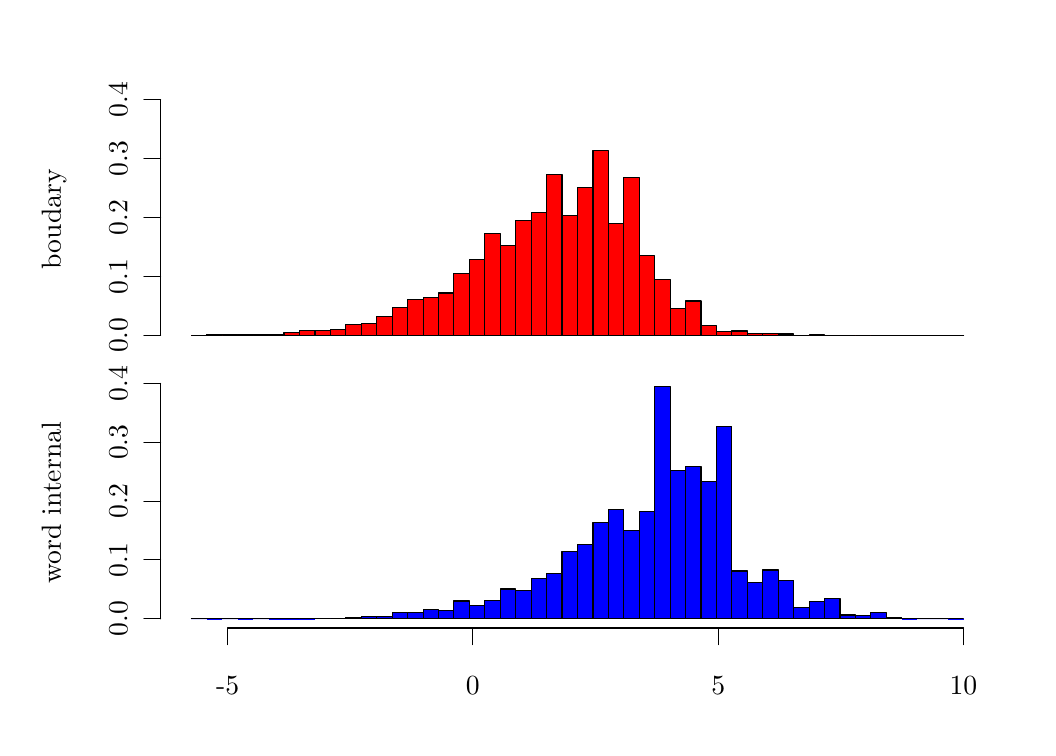
\begin{tikzpicture}[x=1pt,y=1pt]
\definecolor[named]{drawColor}{rgb}{0.00,0.00,0.00}
\definecolor[named]{fillColor}{rgb}{1.00,1.00,1.00}
\fill[color=fillColor,] (0,0) rectangle (361.35,252.94);
\begin{scope}
\path[clip] (  0.00,126.47) rectangle (361.35,252.94);
\definecolor[named]{drawColor}{rgb}{0.78,0.56,0.83}
\definecolor[named]{drawColor}{rgb}{0.00,0.00,0.00}

\node[rotate= 90.00,color=drawColor,anchor=base,inner sep=0pt, outer sep=0pt, scale=  1.00] at ( 12.00,183.71) {boudary%
};
\end{scope}
\begin{scope}
\path[clip] (  0.00,  0.00) rectangle (361.35,252.94);
\definecolor[named]{drawColor}{rgb}{0.78,0.56,0.83}
\definecolor[named]{drawColor}{rgb}{0.00,0.00,0.00}

\draw[color=drawColor,line cap=round,line join=round,fill opacity=0.00,] ( 48.00,141.82) -- ( 48.00,226.87);

\draw[color=drawColor,line cap=round,line join=round,fill opacity=0.00,] ( 48.00,141.82) -- ( 42.00,141.82);

\draw[color=drawColor,line cap=round,line join=round,fill opacity=0.00,] ( 48.00,163.08) -- ( 42.00,163.08);

\draw[color=drawColor,line cap=round,line join=round,fill opacity=0.00,] ( 48.00,184.35) -- ( 42.00,184.35);

\draw[color=drawColor,line cap=round,line join=round,fill opacity=0.00,] ( 48.00,205.61) -- ( 42.00,205.61);

\draw[color=drawColor,line cap=round,line join=round,fill opacity=0.00,] ( 48.00,226.87) -- ( 42.00,226.87);

\node[rotate= 90.00,color=drawColor,anchor=base,inner sep=0pt, outer sep=0pt, scale=  1.00] at ( 36.00,141.82) {0.0%
};

\node[rotate= 90.00,color=drawColor,anchor=base,inner sep=0pt, outer sep=0pt, scale=  1.00] at ( 36.00,163.08) {0.1%
};

\node[rotate= 90.00,color=drawColor,anchor=base,inner sep=0pt, outer sep=0pt, scale=  1.00] at ( 36.00,184.35) {0.2%
};

\node[rotate= 90.00,color=drawColor,anchor=base,inner sep=0pt, outer sep=0pt, scale=  1.00] at ( 36.00,205.61) {0.3%
};

\node[rotate= 90.00,color=drawColor,anchor=base,inner sep=0pt, outer sep=0pt, scale=  1.00] at ( 36.00,226.87) {0.4%
};
\end{scope}
\begin{scope}
\path[clip] ( 48.00,138.47) rectangle (349.35,228.94);
\definecolor[named]{drawColor}{rgb}{0.78,0.56,0.83}
\definecolor[named]{drawColor}{rgb}{0.00,0.00,0.00}
\definecolor[named]{fillColor}{rgb}{1.00,0.00,0.00}

\draw[color=drawColor,line cap=round,line join=round,fill=fillColor,] ( 59.16,141.82) rectangle ( 64.74,141.84);

\draw[color=drawColor,line cap=round,line join=round,fill=fillColor,] ( 64.74,141.82) rectangle ( 70.32,141.92);

\draw[color=drawColor,line cap=round,line join=round,fill=fillColor,] ( 70.32,141.82) rectangle ( 75.90,142.01);

\draw[color=drawColor,line cap=round,line join=round,fill=fillColor,] ( 75.90,141.82) rectangle ( 81.48,141.90);

\draw[color=drawColor,line cap=round,line join=round,fill=fillColor,] ( 81.48,141.82) rectangle ( 87.06,142.11);

\draw[color=drawColor,line cap=round,line join=round,fill=fillColor,] ( 87.06,141.82) rectangle ( 92.64,142.15);

\draw[color=drawColor,line cap=round,line join=round,fill=fillColor,] ( 92.64,141.82) rectangle ( 98.23,142.67);

\draw[color=drawColor,line cap=round,line join=round,fill=fillColor,] ( 98.23,141.82) rectangle (103.81,143.48);

\draw[color=drawColor,line cap=round,line join=round,fill=fillColor,] (103.81,141.82) rectangle (109.39,143.36);

\draw[color=drawColor,line cap=round,line join=round,fill=fillColor,] (109.39,141.82) rectangle (114.97,143.83);

\draw[color=drawColor,line cap=round,line join=round,fill=fillColor,] (114.97,141.82) rectangle (120.55,145.54);

\draw[color=drawColor,line cap=round,line join=round,fill=fillColor,] (120.55,141.82) rectangle (126.13,146.05);

\draw[color=drawColor,line cap=round,line join=round,fill=fillColor,] (126.13,141.82) rectangle (131.71,148.70);

\draw[color=drawColor,line cap=round,line join=round,fill=fillColor,] (131.71,141.82) rectangle (137.29,151.69);

\draw[color=drawColor,line cap=round,line join=round,fill=fillColor,] (137.29,141.82) rectangle (142.87,154.58);

\draw[color=drawColor,line cap=round,line join=round,fill=fillColor,] (142.87,141.82) rectangle (148.45,155.33);

\draw[color=drawColor,line cap=round,line join=round,fill=fillColor,] (148.45,141.82) rectangle (154.03,157.05);

\draw[color=drawColor,line cap=round,line join=round,fill=fillColor,] (154.03,141.82) rectangle (159.61,164.07);

\draw[color=drawColor,line cap=round,line join=round,fill=fillColor,] (159.61,141.82) rectangle (165.19,169.06);

\draw[color=drawColor,line cap=round,line join=round,fill=fillColor,] (165.19,141.82) rectangle (170.77,178.46);

\draw[color=drawColor,line cap=round,line join=round,fill=fillColor,] (170.77,141.82) rectangle (176.35,174.28);

\draw[color=drawColor,line cap=round,line join=round,fill=fillColor,] (176.35,141.82) rectangle (181.93,183.38);

\draw[color=drawColor,line cap=round,line join=round,fill=fillColor,] (181.93,141.82) rectangle (187.51,185.99);

\draw[color=drawColor,line cap=round,line join=round,fill=fillColor,] (187.51,141.82) rectangle (193.09,200.00);

\draw[color=drawColor,line cap=round,line join=round,fill=fillColor,] (193.09,141.82) rectangle (198.68,185.18);

\draw[color=drawColor,line cap=round,line join=round,fill=fillColor,] (198.68,141.82) rectangle (204.26,195.27);

\draw[color=drawColor,line cap=round,line join=round,fill=fillColor,] (204.26,141.82) rectangle (209.84,208.55);

\draw[color=drawColor,line cap=round,line join=round,fill=fillColor,] (209.84,141.82) rectangle (215.42,182.19);

\draw[color=drawColor,line cap=round,line join=round,fill=fillColor,] (215.42,141.82) rectangle (221.00,198.65);

\draw[color=drawColor,line cap=round,line join=round,fill=fillColor,] (221.00,141.82) rectangle (226.58,170.46);

\draw[color=drawColor,line cap=round,line join=round,fill=fillColor,] (226.58,141.82) rectangle (232.16,161.80);

\draw[color=drawColor,line cap=round,line join=round,fill=fillColor,] (232.16,141.82) rectangle (237.74,151.51);

\draw[color=drawColor,line cap=round,line join=round,fill=fillColor,] (237.74,141.82) rectangle (243.32,154.18);

\draw[color=drawColor,line cap=round,line join=round,fill=fillColor,] (243.32,141.82) rectangle (248.90,145.36);

\draw[color=drawColor,line cap=round,line join=round,fill=fillColor,] (248.90,141.82) rectangle (254.48,143.30);

\draw[color=drawColor,line cap=round,line join=round,fill=fillColor,] (254.48,141.82) rectangle (260.06,143.34);

\draw[color=drawColor,line cap=round,line join=round,fill=fillColor,] (260.06,141.82) rectangle (265.64,142.39);

\draw[color=drawColor,line cap=round,line join=round,fill=fillColor,] (265.64,141.82) rectangle (271.22,142.51);

\draw[color=drawColor,line cap=round,line join=round,fill=fillColor,] (271.22,141.82) rectangle (276.80,142.25);

\draw[color=drawColor,line cap=round,line join=round,fill=fillColor,] (276.80,141.82) rectangle (282.38,141.82);

\draw[color=drawColor,line cap=round,line join=round,fill=fillColor,] (282.38,141.82) rectangle (287.96,141.88);

\draw[color=drawColor,line cap=round,line join=round,fill=fillColor,] (287.96,141.82) rectangle (293.54,141.82);

\draw[color=drawColor,line cap=round,line join=round,fill=fillColor,] (293.54,141.82) rectangle (299.12,141.82);

\draw[color=drawColor,line cap=round,line join=round,fill=fillColor,] (299.12,141.82) rectangle (304.71,141.86);

\draw[color=drawColor,line cap=round,line join=round,fill=fillColor,] (304.71,141.82) rectangle (310.29,141.82);

\draw[color=drawColor,line cap=round,line join=round,fill=fillColor,] (310.29,141.82) rectangle (315.87,141.82);

\draw[color=drawColor,line cap=round,line join=round,fill=fillColor,] (315.87,141.82) rectangle (321.45,141.82);

\draw[color=drawColor,line cap=round,line join=round,fill=fillColor,] (321.45,141.82) rectangle (327.03,141.82);

\draw[color=drawColor,line cap=round,line join=round,fill=fillColor,] (327.03,141.82) rectangle (332.61,141.82);

\draw[color=drawColor,line cap=round,line join=round,fill=fillColor,] (332.61,141.82) rectangle (338.19,141.82);
\end{scope}
\begin{scope}
\path[clip] ( 48.00, 36.00) rectangle (349.35,126.47);
\definecolor[named]{drawColor}{rgb}{0.78,0.56,0.83}
\end{scope}
\begin{scope}
\path[clip] (  0.00,  0.00) rectangle (361.35,126.47);
\definecolor[named]{drawColor}{rgb}{0.78,0.56,0.83}
\definecolor[named]{drawColor}{rgb}{0.00,0.00,0.00}

\node[rotate= 90.00,color=drawColor,anchor=base,inner sep=0pt, outer sep=0pt, scale=  1.00] at ( 12.00, 81.24) {word internal%
};
\end{scope}
\begin{scope}
\path[clip] (  0.00,  0.00) rectangle (361.35,252.94);
\definecolor[named]{drawColor}{rgb}{0.78,0.56,0.83}
\definecolor[named]{drawColor}{rgb}{0.00,0.00,0.00}

\draw[color=drawColor,line cap=round,line join=round,fill opacity=0.00,] ( 72.24, 36.00) -- (338.15, 36.00);

\draw[color=drawColor,line cap=round,line join=round,fill opacity=0.00,] ( 72.24, 36.00) -- ( 72.24, 30.00);

\draw[color=drawColor,line cap=round,line join=round,fill opacity=0.00,] (160.88, 36.00) -- (160.88, 30.00);

\draw[color=drawColor,line cap=round,line join=round,fill opacity=0.00,] (249.51, 36.00) -- (249.51, 30.00);

\draw[color=drawColor,line cap=round,line join=round,fill opacity=0.00,] (338.15, 36.00) -- (338.15, 30.00);

\node[color=drawColor,anchor=base,inner sep=0pt, outer sep=0pt, scale=  1.00] at ( 72.24, 12.00) {-5%
};

\node[color=drawColor,anchor=base,inner sep=0pt, outer sep=0pt, scale=  1.00] at (160.88, 12.00) {0%
};

\node[color=drawColor,anchor=base,inner sep=0pt, outer sep=0pt, scale=  1.00] at (249.51, 12.00) {5%
};

\node[color=drawColor,anchor=base,inner sep=0pt, outer sep=0pt, scale=  1.00] at (338.15, 12.00) {10%
};

\draw[color=drawColor,line cap=round,line join=round,fill opacity=0.00,] ( 48.00, 39.35) -- ( 48.00,124.40);

\draw[color=drawColor,line cap=round,line join=round,fill opacity=0.00,] ( 48.00, 39.35) -- ( 42.00, 39.35);

\draw[color=drawColor,line cap=round,line join=round,fill opacity=0.00,] ( 48.00, 60.61) -- ( 42.00, 60.61);

\draw[color=drawColor,line cap=round,line join=round,fill opacity=0.00,] ( 48.00, 81.87) -- ( 42.00, 81.87);

\draw[color=drawColor,line cap=round,line join=round,fill opacity=0.00,] ( 48.00,103.14) -- ( 42.00,103.14);

\draw[color=drawColor,line cap=round,line join=round,fill opacity=0.00,] ( 48.00,124.40) -- ( 42.00,124.40);

\node[rotate= 90.00,color=drawColor,anchor=base,inner sep=0pt, outer sep=0pt, scale=  1.00] at ( 36.00, 39.35) {0.0%
};

\node[rotate= 90.00,color=drawColor,anchor=base,inner sep=0pt, outer sep=0pt, scale=  1.00] at ( 36.00, 60.61) {0.1%
};

\node[rotate= 90.00,color=drawColor,anchor=base,inner sep=0pt, outer sep=0pt, scale=  1.00] at ( 36.00, 81.87) {0.2%
};

\node[rotate= 90.00,color=drawColor,anchor=base,inner sep=0pt, outer sep=0pt, scale=  1.00] at ( 36.00,103.14) {0.3%
};

\node[rotate= 90.00,color=drawColor,anchor=base,inner sep=0pt, outer sep=0pt, scale=  1.00] at ( 36.00,124.40) {0.4%
};
\end{scope}
\begin{scope}
\path[clip] ( 48.00, 36.00) rectangle (349.35,126.47);
\definecolor[named]{drawColor}{rgb}{0.78,0.56,0.83}
\definecolor[named]{drawColor}{rgb}{0.00,0.00,0.00}
\definecolor[named]{fillColor}{rgb}{0.00,0.00,1.00}

\draw[color=drawColor,line cap=round,line join=round,fill=fillColor,] ( 59.16, 39.35) rectangle ( 64.74, 39.35);

\draw[color=drawColor,line cap=round,line join=round,fill=fillColor,] ( 64.74, 39.35) rectangle ( 70.32, 39.38);

\draw[color=drawColor,line cap=round,line join=round,fill=fillColor,] ( 70.32, 39.35) rectangle ( 75.90, 39.35);

\draw[color=drawColor,line cap=round,line join=round,fill=fillColor,] ( 75.90, 39.35) rectangle ( 81.48, 39.36);

\draw[color=drawColor,line cap=round,line join=round,fill=fillColor,] ( 81.48, 39.35) rectangle ( 87.06, 39.35);

\draw[color=drawColor,line cap=round,line join=round,fill=fillColor,] ( 87.06, 39.35) rectangle ( 92.64, 39.40);

\draw[color=drawColor,line cap=round,line join=round,fill=fillColor,] ( 92.64, 39.35) rectangle ( 98.23, 39.43);

\draw[color=drawColor,line cap=round,line join=round,fill=fillColor,] ( 98.23, 39.35) rectangle (103.81, 39.44);

\draw[color=drawColor,line cap=round,line join=round,fill=fillColor,] (103.81, 39.35) rectangle (109.39, 39.49);

\draw[color=drawColor,line cap=round,line join=round,fill=fillColor,] (109.39, 39.35) rectangle (114.97, 39.59);

\draw[color=drawColor,line cap=round,line join=round,fill=fillColor,] (114.97, 39.35) rectangle (120.55, 39.65);

\draw[color=drawColor,line cap=round,line join=round,fill=fillColor,] (120.55, 39.35) rectangle (126.13, 40.23);

\draw[color=drawColor,line cap=round,line join=round,fill=fillColor,] (126.13, 39.35) rectangle (131.71, 40.31);

\draw[color=drawColor,line cap=round,line join=round,fill=fillColor,] (131.71, 39.35) rectangle (137.29, 41.47);

\draw[color=drawColor,line cap=round,line join=round,fill=fillColor,] (137.29, 39.35) rectangle (142.87, 41.46);

\draw[color=drawColor,line cap=round,line join=round,fill=fillColor,] (142.87, 39.35) rectangle (148.45, 42.63);

\draw[color=drawColor,line cap=round,line join=round,fill=fillColor,] (148.45, 39.35) rectangle (154.03, 42.28);

\draw[color=drawColor,line cap=round,line join=round,fill=fillColor,] (154.03, 39.35) rectangle (159.61, 45.78);

\draw[color=drawColor,line cap=round,line join=round,fill=fillColor,] (159.61, 39.35) rectangle (165.19, 44.08);

\draw[color=drawColor,line cap=round,line join=round,fill=fillColor,] (165.19, 39.35) rectangle (170.77, 46.06);

\draw[color=drawColor,line cap=round,line join=round,fill=fillColor,] (170.77, 39.35) rectangle (176.35, 50.12);

\draw[color=drawColor,line cap=round,line join=round,fill=fillColor,] (176.35, 39.35) rectangle (181.93, 49.71);

\draw[color=drawColor,line cap=round,line join=round,fill=fillColor,] (181.93, 39.35) rectangle (187.51, 53.74);

\draw[color=drawColor,line cap=round,line join=round,fill=fillColor,] (187.51, 39.35) rectangle (193.09, 55.69);

\draw[color=drawColor,line cap=round,line join=round,fill=fillColor,] (193.09, 39.35) rectangle (198.68, 63.62);

\draw[color=drawColor,line cap=round,line join=round,fill=fillColor,] (198.68, 39.35) rectangle (204.26, 66.09);

\draw[color=drawColor,line cap=round,line join=round,fill=fillColor,] (204.26, 39.35) rectangle (209.84, 74.08);

\draw[color=drawColor,line cap=round,line join=round,fill=fillColor,] (209.84, 39.35) rectangle (215.42, 78.93);

\draw[color=drawColor,line cap=round,line join=round,fill=fillColor,] (215.42, 39.35) rectangle (221.00, 71.40);

\draw[color=drawColor,line cap=round,line join=round,fill=fillColor,] (221.00, 39.35) rectangle (226.58, 78.16);

\draw[color=drawColor,line cap=round,line join=round,fill=fillColor,] (226.58, 39.35) rectangle (232.16,123.12);

\draw[color=drawColor,line cap=round,line join=round,fill=fillColor,] (232.16, 39.35) rectangle (237.74, 92.77);

\draw[color=drawColor,line cap=round,line join=round,fill=fillColor,] (237.74, 39.35) rectangle (243.32, 94.51);

\draw[color=drawColor,line cap=round,line join=round,fill=fillColor,] (243.32, 39.35) rectangle (248.90, 88.91);

\draw[color=drawColor,line cap=round,line join=round,fill=fillColor,] (248.90, 39.35) rectangle (254.48,108.84);

\draw[color=drawColor,line cap=round,line join=round,fill=fillColor,] (254.48, 39.35) rectangle (260.06, 56.61);

\draw[color=drawColor,line cap=round,line join=round,fill=fillColor,] (260.06, 39.35) rectangle (265.64, 52.55);

\draw[color=drawColor,line cap=round,line join=round,fill=fillColor,] (265.64, 39.35) rectangle (271.22, 56.95);

\draw[color=drawColor,line cap=round,line join=round,fill=fillColor,] (271.22, 39.35) rectangle (276.80, 53.26);

\draw[color=drawColor,line cap=round,line join=round,fill=fillColor,] (276.80, 39.35) rectangle (282.38, 43.44);

\draw[color=drawColor,line cap=round,line join=round,fill=fillColor,] (282.38, 39.35) rectangle (287.96, 45.56);

\draw[color=drawColor,line cap=round,line join=round,fill=fillColor,] (287.96, 39.35) rectangle (293.54, 46.60);

\draw[color=drawColor,line cap=round,line join=round,fill=fillColor,] (293.54, 39.35) rectangle (299.12, 40.71);

\draw[color=drawColor,line cap=round,line join=round,fill=fillColor,] (299.12, 39.35) rectangle (304.71, 40.52);

\draw[color=drawColor,line cap=round,line join=round,fill=fillColor,] (304.71, 39.35) rectangle (310.29, 41.54);

\draw[color=drawColor,line cap=round,line join=round,fill=fillColor,] (310.29, 39.35) rectangle (315.87, 39.92);

\draw[color=drawColor,line cap=round,line join=round,fill=fillColor,] (315.87, 39.35) rectangle (321.45, 39.38);

\draw[color=drawColor,line cap=round,line join=round,fill=fillColor,] (321.45, 39.35) rectangle (327.03, 39.35);

\draw[color=drawColor,line cap=round,line join=round,fill=fillColor,] (327.03, 39.35) rectangle (332.61, 39.35);

\draw[color=drawColor,line cap=round,line join=round,fill=fillColor,] (332.61, 39.35) rectangle (338.19, 39.37);
\end{scope}
\end{tikzpicture}
